\documentclass[../main.tex]{subfiles}

\begin{document}
\section{Introduction to astrodynamics and satellite tracking}
\subsection{The two body problem}\label{sec:twoBody}
\subsubsection{Trajectory equation}
We are interested in understanding the dynamics of a spacecraft in orbit around the Earth. These dynamics are governed by Newton's second law of motion, which assuming that both the Earth and the spacecraft are point masses (see \cref{sec:force} for a more realistic model), this can be written as
\begin{equation}
  \label{eq:Newton}
  \ddot{\vf{r}}=-\frac{GM_{\oplus}}{r^2}\vf{e}_r
\end{equation}
where $\vf{r}$ is the position vector (also called \emph{radius vector}) of the spacecraft with respect to the center of the Earth, $r:=\norm{\vf{r}}$, $\vf{e}_r=\frac{\vf{r}}{r}$ is the unit vector in the direction of $\vf{r}$, $M_{\oplus}\simeq 5.972\times 10^{24}\ \kg$ is the mass of the Earth, and $G\simeq 6.674\times 10^{-11}\ \m^3\cdot \kg^{-1}\cdot\s^{-2}$ is the universal gravitational constant. Note that the minus sign is due to the fact that the gravitational force is attractive, i.e.\ pointing towards the Earth.
Here and throughout the document the \emph{dot notation} $\ddot{\vf{r}}$ means that the derivatives are taken with respect to time.
Cross-multiplying \cref{eq:Newton} by $\vf{r}$, we obtain
\begin{equation}
  \dv{(\vf{r}\times \dot{\vf{r}})}{t}=\dot{\vf{r}}\times \dot{\vf{r}}+\vf{r}\times\ddot{\vf{r}}=-\frac{GM_{\oplus}}{r^3}(\vf{r}\times \vf{r})=0
\end{equation}
Hence $\vf{h}:=\vf{r}\times \dot{\vf{r}}$ is constant. The physical intuition behind this is that the motion of the spacecraft around the Earth is confined to a plane, called the \emph{orbital plane}, because the position $\vf{r}$ and velocity $\dot{\vf{r}}$ are always perpendicular to $\vf{h}$.

We are interested now in what kind of curves may be described by a spacecraft orbiting the Earth, when considered both objects as point masses. That is, we want to somehow isolate $\vf{r}$ (or $r$) from \cref{eq:Newton}. In order to simplify the notation we will denote $\mu:=GM_{\oplus}$.
\begin{proposition}[Kepler's first law]
  \label{prop:two-body}
  Consider two point-mass bodies. The motion of one body orbiting the other can be described by a conic section. Hence, it can be expressed in the form:
  \begin{equation}
    \label{eq:two-body}
    r(t)=\frac{p}{1+e\cos (\nu(t))}
  \end{equation}
  for some parameters $p$ and $e$.
\end{proposition}
\begin{proof}
  Cross-multiplying \cref{eq:Newton} by $\vf{h}$ we obtain
  \begin{equation}\label{eq:rtimesh}
    \dv{(\dot{\vf{r}}\times\vf{h})}{t}=\ddot{\vf{r}}\times\vf{h}=-\frac{\mu}{r^3}\vf{r}\times\vf{h}=-\frac{\mu}{r^3}\vf{r}\times(\vf{r}\times \dot{\vf{r}})=\frac{\mu}{r^3}[(\vf{r}\cdot{\vf{r}})\dot{\vf{r}}-(\vf{r}\cdot\dot{\vf{r}})\vf{r}]
  \end{equation}
  where in the last equality we have used the vector equality $\vf{u}\times(\vf{v}\times\vf{w})=(\vf{u}\cdot\vf{w})\vf{v}-(\vf{u}\cdot\vf{v})\vf{w}$ for $\vf{u}, \vf{v}, \vf{w}\in\RR^3$. Now note that:
  \begin{equation}
    \dv{}{t}\left(\frac{\vf{r}}{r}\right)=\frac{\dot{\vf{r}}}{r}-\frac{\dot{r}}{r^2}\vf{r}= \frac{1}{r^3}[(\vf{r}\cdot{\vf{r}})\dot{\vf{r}}-(\vf{r}\cdot\dot{\vf{r}})\vf{r}]
  \end{equation}
  because\footnote{Bear in mind that in general $\dot{r}\ne\norm{\dot{\vf{r}}}$. Indeed, if $\beta$ denotes the angle between $\vf{r}$ and $\dot{\vf{r}}$ we have that $\dot{r}=\norm{\dot{\vf{r}}}\cos\beta$. In particular $\dot{r}$ may be negative.} $\displaystyle 2r\dot{r}=\dv{(r^2)}{t}=\dv{(\vf{r}\cdot\vf{r})}{t}=2\vf{r}\cdot\dot{\vf{r}}$. Thus:
  \begin{equation}
    \dv{(\dot{\vf{r}}\times\vf{h})}{t}=\mu \dv{}{t}\left(\frac{\vf{r}}{r}\right)
  \end{equation}
  Integrating with respect to the time yields
  \begin{equation}\label{eq:rdottimesh}
    \dot{\vf{r}}\times \vf{h}=\frac{\mu}{r}\vf{r}+\vf{B}
  \end{equation}
  where $\vf{B}\in\RR^3$ is the constant of integration. Observe that since $\dot{\vf{r}}\times\vf{h}$ is perpendicular to $\vf{h}$, $\dot{\vf{r}}\times\vf{h}$ lies on the orbital plane and so does $\vf{r}$. Hence, $\vf{B}$ lies on the orbital plane too. Now, dot-multiplying this last equation by $\vf{r}$ and using that $\vf{u}\cdot(\vf{v}\times\vf{w})=(\vf{u}\times\vf{v})\cdot\vf{w}$ $\forall\vf{u},\vf{v},\vf{w}\in\RR^3$ we obtain
  \begin{equation}
    h^2=\vf{h}\cdot\vf{h}=(\vf{r}\times\dot{\vf{r}})\cdot\vf{h}=\vf{r}\cdot(\dot{\vf{r}}\times\vf{h})=\frac{\mu}{r}\vf{r}\cdot\vf{r}+\vf{r}\cdot\vf{B}=\mu r+rB\cos\nu
  \end{equation}
  where $h:=\norm{\vf{h}}$, $B:=\norm{\vf{B}}$ and $\nu$ denotes the angle between $\vf{r}$ and $\vf{B}$, called \emph{true anomaly}. Rearranging the terms we finally obtain the equation of a conic section
  \begin{equation}\label{eq:r_conic}
    r=\frac{h^2/\mu}{1+(B/\mu)\cos(\nu)}
  \end{equation}
  with $p:=h^2/\mu$ and $e:=B/\mu$.
\end{proof}
From here on, let's assume that $B$ is small enough to satisfy $e <1$, as this is the primary case of interest. We've seen in \cref{sec:ellipse} the range of values that can $r$ take in that case, and we deduced an equation for the semi-major axis. Note that this latter quantity can also be expressed as:
\begin{equation}\label{eq:semi-major_axis}
  a=\frac{r_\mathrm{max}+r_\mathrm{min}}{2}=\frac{p}{1-e^2}=\frac{h^2}{\mu(1-e^2)}
\end{equation}
Note that at $\vf{r}_\mathrm{min}$, we have $\nu=0$ and so $\vf{r}\parallel\vf{B}$. Hence, $\vf{B}$ points towards the periapsis of the orbit.
\begin{definition}
  Let $\vf{r}(t)$ be the position of the spacecraft at time $t$ and $A(t)$ be the area swept by the radius vector $\vf{r}(t)$ in the time interval $[0,t]$. We define the \emph{areal velocity} as $\dv{A(t)}{t}$.
\end{definition}
\begin{proposition}[Kepler's second law]
  The areal velocity remains constant.
\end{proposition}
\begin{proof}
  Recall that the area of a parallelogram generated by two vectors $\vf{u},\vf{v}\in\RR^3$ is given by $\norm{\vf{u}\times\vf{v}}$. Thus, approximating the difference $A(t+k)-A(t)$ by half of the area of the parallelogram generated by $\vf{r}(t)$ and ${\vf{r}}(t+k)$ (see \cref{fig:areal_vel}) we obtain:
  \begin{multline}\label{eq:areal_velocity}
    \dv{A(t)}{t}=\lim_{k\to 0}\frac{A(t+k)-A(t)}{k}=\lim_{k\to 0}\frac{\norm{\vf{r}(t)\times\vf{r}(t+k)}}{2k}=\lim_{k\to 0}\frac{\norm{\vf{r}(t)\times(\vf{r}(t+k)-\vf{r}(t))}}{2k}=\\
    =\frac{\norm{\vf{r}(t)\times\dot{\vf{r}}(t)}}{2}=\frac{h}{2}
  \end{multline}
  where the penultimate equality is due to the continuity and linearity of the cross product.
\end{proof}
\begin{figure}[htbp]
  \centering
  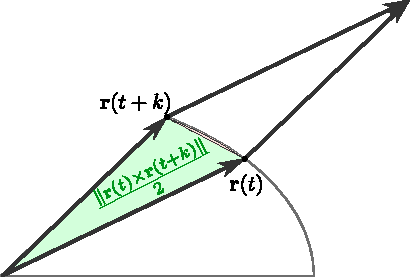
\includegraphics[width=0.5\textwidth]{Images/areal_velocity.pdf}
  \caption{Graphical representation of the error made (red region) when approximating the area swept by the radius vector by half the area of the parallelogram generated by $\vf{r}(t)$ and $\vf{r}(t+k)$ (green region).}
  \label{fig:areal_vel}
\end{figure}
\begin{definition}
  Let $T$ be the orbital period of the satellite. We define the \emph{mean motion} as $n:=2\pi/T$.
\end{definition}
\begin{proposition}[Kepler's third law]\label{prop:kepler_third_law}
  The mean motion is related to the semi-major axis by:
  \begin{equation}
    n=\sqrt{\frac{\mu}{a^3}}
  \end{equation}
\end{proposition}
\begin{proof}
  Integrating \cref{eq:areal_velocity} with respect to time between 0 and $T$ (the period) yields:
  \begin{equation}
    \pi a b=A(T)=\int_0^T A'(t)\dd{t}=\int_0^T \frac{h}{2}\dd{t}=\frac{hT}{2}\implies n=\frac{2\pi}{T}=\frac{h}{a b}=\frac{h}{a^2\sqrt{1-e^2}}=\sqrt{\frac{\mu}{a^3}}
  \end{equation}
  where we have used \cref{eq:semi-major_axis,eq:ellipse_b_a}.
\end{proof}
% \textcolor{red}{Finally we will need the following equation which relates the velocity of the satellite with the distance to the central of the Earth.
%   \begin{proposition}
%     We have that (\cite{montenbruck}):
%     \begin{equation}\label{eq:visviva}
%       v^2=\mu\left(\frac{2}{r}-\frac{1}{a}\right)
%     \end{equation}
%     where $v:=\norm{\dot{\vf{r}}}$.
%   \end{proposition}
%   \begin{proof}
%     Using \cref{eq:rdottimesh} we have that:
%     \begin{equation}
%       \norm{\vf{h}\times\dot{\vf{r}}}^2=\frac{\mu^2}{r^2}\vf{r}\cdot\vf{r}+2\frac{\mu}{r}\vf{r}\cdot\vf{B}+\vf{B} \cdot \vf{B}=\mu^2(1+2 e\cos\nu + e^2)=\mu^2(2(1+ e\cos\nu) -(1- e^2))
%     \end{equation}
%     where we have used that $e\mu=B$ (see \cref{eq:r_conic}). Now using \cref{eq:r_conic,eq:semi-major_axis} we obtain that
%     \begin{equation}
%       2(1+ e\cos\nu) -(1- e^2)=2\frac{p}{r}-\frac{h^2}{\mu a}=2\frac{h^2}{r\mu}-\frac{h^2}{\mu a}
%     \end{equation}
%     Since $\vf{h}\perp\dot{\vf{r}}$, $\norm{\vf{h}\times\dot{\vf{r}}}=hv$ and so:
%     \begin{equation}
%       v^2=\mu\left(\frac{2}{r}-\frac{1}{a}\right)
%     \end{equation}
%   \end{proof}}
\subsubsection{Kepler's equation}\label{sec:kepler_equation}
So far we have been able to describe the geometry of motion of a body orbiting another one. However, we have not concerned about the specific position of the body as a function of time. That is how to obtain $\nu(t)$ at each instant of time. In order to do this, we may think the area $A$ as a function of $\nu$, that measures the area swept by the radio vector from an initial instant $\nu_0$. Thus, from differential calculus we know that:
\begin{equation}
  A(\nu)=\int_{\nu_0}^{\nu}\int_{0}^{r(\theta)}r\dd{r}\dd{\theta}=\int_{\nu_0}^{\nu}\frac{{r(\theta)}^2}{2}\dd{\theta}\implies\dv{A}{\nu}=\frac{r^2}{2}
\end{equation}
Using the chain rule and \cref{eq:areal_velocity} we obtain that:
\begin{equation}\label{eq:areal_velocity_nu}
  \frac{h}{2}=\dv{A}{t}=\dv{A}{\nu}\dv{\nu}{t}=\frac{r^2}{2}\dot\nu
\end{equation}
So from \cref{eq:r_conic,eq:areal_velocity_nu}, we get the following differential equation that must satisfy $\nu$:
\begin{equation}
  \dot\nu=\frac{h}{r^2}=\frac{h}{p^2}{(1+e\cos\nu)}^2
\end{equation}
which, when integrated with respect to the time, lead us to an elliptic integral which can be very computationally expensive. Our goal in this section is to find an easier way to compute the exact position of the satellite at each instant of time \cite{montenbruck}. This will lead us to the so-called \emph{Kepler's equation}. For this purpose we are forced to introduce a new parameter, $E$, called \emph{eccentric anomaly}. It is defined as the angle between the segment from the origin of the ellipse to the periapsis, and the line passing through the center of the ellipse and the point in a circle (of radius $a$ and same center as the ellipse) which is just above the position of the satellite (see \cref{fig:kepler_eq} for a better understanding).
\begin{figure}[ht]
  \centering
  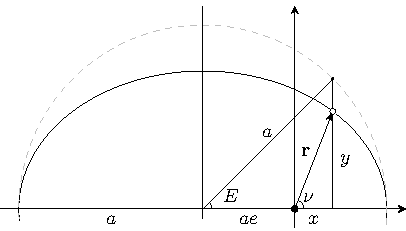
\includegraphics[width=0.5\textwidth]{Images/kepler_eq.pdf}
  \caption{Ellipse orbit of the satellite together with an auxiliary circle of radius $a$ needed to define the eccentric anomaly.}
  \label{fig:kepler_eq}
\end{figure}
Clearly, using the reference frame of \cref{fig:kepler_eq}, the position of the satellite is determined by $x=r\cos\nu$, $y=r\sin\nu$. But we would like to find an expression of $x$ and $y$ in terms of $E$ rather than $\nu$. To do this, note that $a\cos E=ae+x$, so:
\begin{equation}\label{eq:eccentricX}
  x=a(\cos E-e)
\end{equation}
We can also get an expression of $r$ in terms of $E$ by solving the equation:
\begin{equation}\label{eq:eccentricr}
  r=\frac{p}{1+e\cos \nu}=\frac{a(1-e^2)}{1+e\frac{x}{r}}=\frac{ra(1-e^2)}{r+ae(\cos E-e)}\implies r= a(1-e\cos E)
\end{equation}
Finally from \cref{eq:eccentricX,eq:eccentricr} we get:
\begin{equation}
  y^2=r^2-x^2=a^2(1-e^2){(\sin E)}^2\implies y=a\sqrt{1-e^2}\sin E
\end{equation}
Expressing now the areal velocity $h$ as a function of $E$ we have:
\begin{align}
  h & =x\dot{y}-y\dot{x}                                                           \\
    & =a^2(\cos E-e)\sqrt{1-e^2}(\cos E)\dot{E}+a^2{(\sin E)}^2\dot{E}\sqrt{1-e^2} \\
    & =a^2\sqrt{1-e^2}\dot{E}(1-e\cos E)
\end{align}
From \cref{eq:semi-major_axis} we know that $h=\sqrt{\mu a(1-e^2)}$. Thus, substituting this in the latter equation we deduce that $E$ must satisfy the following differential equation:
\begin{equation}\label{eq:kepler_equation_differential}
  \dot{E}(1-e\cos E)=\sqrt{\frac{\mu}{a^3}}=n
\end{equation}
where the last equality follows from \cref{prop:kepler_third_law}. Integrating this equation with respect to time yields the \emph{Kepler's equation}:
\begin{equation}\label{eq:kepler_equation}
  E(t)-e\sin E(t)=n(t-t_0)
\end{equation}
where $t_0$ is the time at which $E$ vanishes. Using the reference frame of \cref{fig:kepler_eq} (also known as the perifocal frame, see \cref{def:perifocal_coordinate_system}) this corresponds to the time at which the satellite is at the perigee. The value $M:=n(t-t_0)$ is called \emph{mean anomaly}. Note that contrarily to $E$ and $\nu$, the mean anomaly increases linearly with time.

Kepler's equation is the key to solve the problem of finding the position of the satellite at each instant of time. Later on we will discuss techniques to effectively solve this equation for $E$, given $e$ and $M$.

\subsection{Time and reference systems}
\subsubsection{Julian day}\label{sec:julian_day}
The measurement of time has undergone significant changes throughout the centuries, and its interpretation continues to vary across different cultures. Astronomy, however, has always needed a universal time measurement system and easy-to-work with. In view of this, the so-called \emph{Julian date} is used as the standard day-counting system in astronomy.
\begin{definition}[Julian date]
  The \emph{Julian date} (JD) is the number of days, of length $24\cdot3600 = 86400$ seconds, elapsed since the beginning of the \emph{Julian period}, that is, since January 1st, 4713 BC at 12:00 (noon) in the Julian calendar\footnote{According to \cite{vallado}, the convention to start the JD at noon each day benefits astronomers (who often work at night) because they can make all their observations on a single day.}. A \emph{Julian year} is defined as 365.25 days and therefore a \emph{Julian century} as 36525 days.
\end{definition}
As the unit of second is not constant among the time systems that we will use throughout the document (UT1, TT, UTC, etc.) (see \cref{sec:time_measurement}), as a consequence, the JD will vary depending on the time system used. We will distinguish them by adding a subscript to the JD, for instance $\text{JD}_\mathrm{UT1}$, $\text{JD}_\mathrm{TT}$ or $\text{JD}_\mathrm{UTC}$. Later on, we will give formulas that relate these time systems, and usually they will be expressed as the number of Julian centuries elapsed since January 1st, 2000 at 12:00 TT (noon) in the Julian calendar. This number is given by:
\begin{equation}
  \frac{\text{JD}-2451545}{36525}
\end{equation}
Here 2451545 corresponds to the Julian date of January 1st, 2000 at 12:00 TT (noon).
\subsubsection{Time measurement}\label{sec:time_measurement}
As human beings, we are naturally interested in how time passes and therefore the correct measure of it becomes an essential necessity for us. As it is the Sun that governs our daily activity, it is natural to define time from it.
But first we need some preliminary definitions:
\begin{definition}
  We define the \emph{equatorial plane} as the plane in $\RR^3$ that contains the Earth equator. We define the \emph{ecliptic plane} as the orbital plane in $\RR^3$ of the Earth around the Sun.
\end{definition}
\begin{definition}
  We define the \emph{celestial sphere} as an abstract sphere of infinite radius centered at the center of mass of the Earth. All the celestial objects are thus, projected naturally on the celestial sphere, identifying them with two spherical coordinates, known as \emph{right ascension} and \emph{declination}, which we define below. The intersection of the equatorial plane with the celestial sphere is called \emph{celestial equator}. The intersection of the ecliptic plane with the celestial sphere is called \emph{ecliptic} (see \cref{fig:right_ascesion} for a better understanding).
\end{definition}
A first important thing to note is that, since the celestial sphere is centered at the Earth, the Sun moves along the ecliptic. Moreover, note that both the celestial equator and the ecliptic are two different great circles on the celestial sphere. Hence, they intersect at exactly two points.

\begin{definition}
  Consider the two points of intersection between the celestial equator and the ecliptic. We define the \emph{vernal equinox} as the point $\Upsilon$, from these two, where the Sun crosses the celestial equator from south to north.
\end{definition}
The angle measured along the equator of any object on the celestial sphere from the vernal equinox is called \emph{right ascension}, whereas the angle measured along the meridian of the object from the position of the object to the equator is called \emph{declination} (see \cref{fig:right_ascesion}).

An \emph{apparent solar day} is defined to be the time between two successive transits of the Sun across our local meridian. One should note that the Earth has to rotate on itself slightly more than one revolution in order to complete one solar day. In addition, due to the non-circular orbit of the Earth around the Sun, the length of an apparent solar day is not constant, as the Earth has to rotate on itself slightly more in the perihelion that in the aphelion. The \emph{apparent sidereal day} is defined as the time it takes for the Earth to complete a rotation (see \cref{fig:sidereal} for a better understanding). From the point of view of the celestial sphere, the apparent solar time is the angle (measured along the celestial equator) between the local meridian\footnote{We consider the local meridian as the meridian on the celestial sphere that is projected onto the Earth and moves in synchronization with it.} and the meridian of the Sun at that epoch, which is not uniform because the angular velocity of the Earth is not constant \cite{montenbruck}.

\begin{figure}[htbp]
  \centering
  \begin{minipage}[ht]{0.47\textwidth}
    \centering
    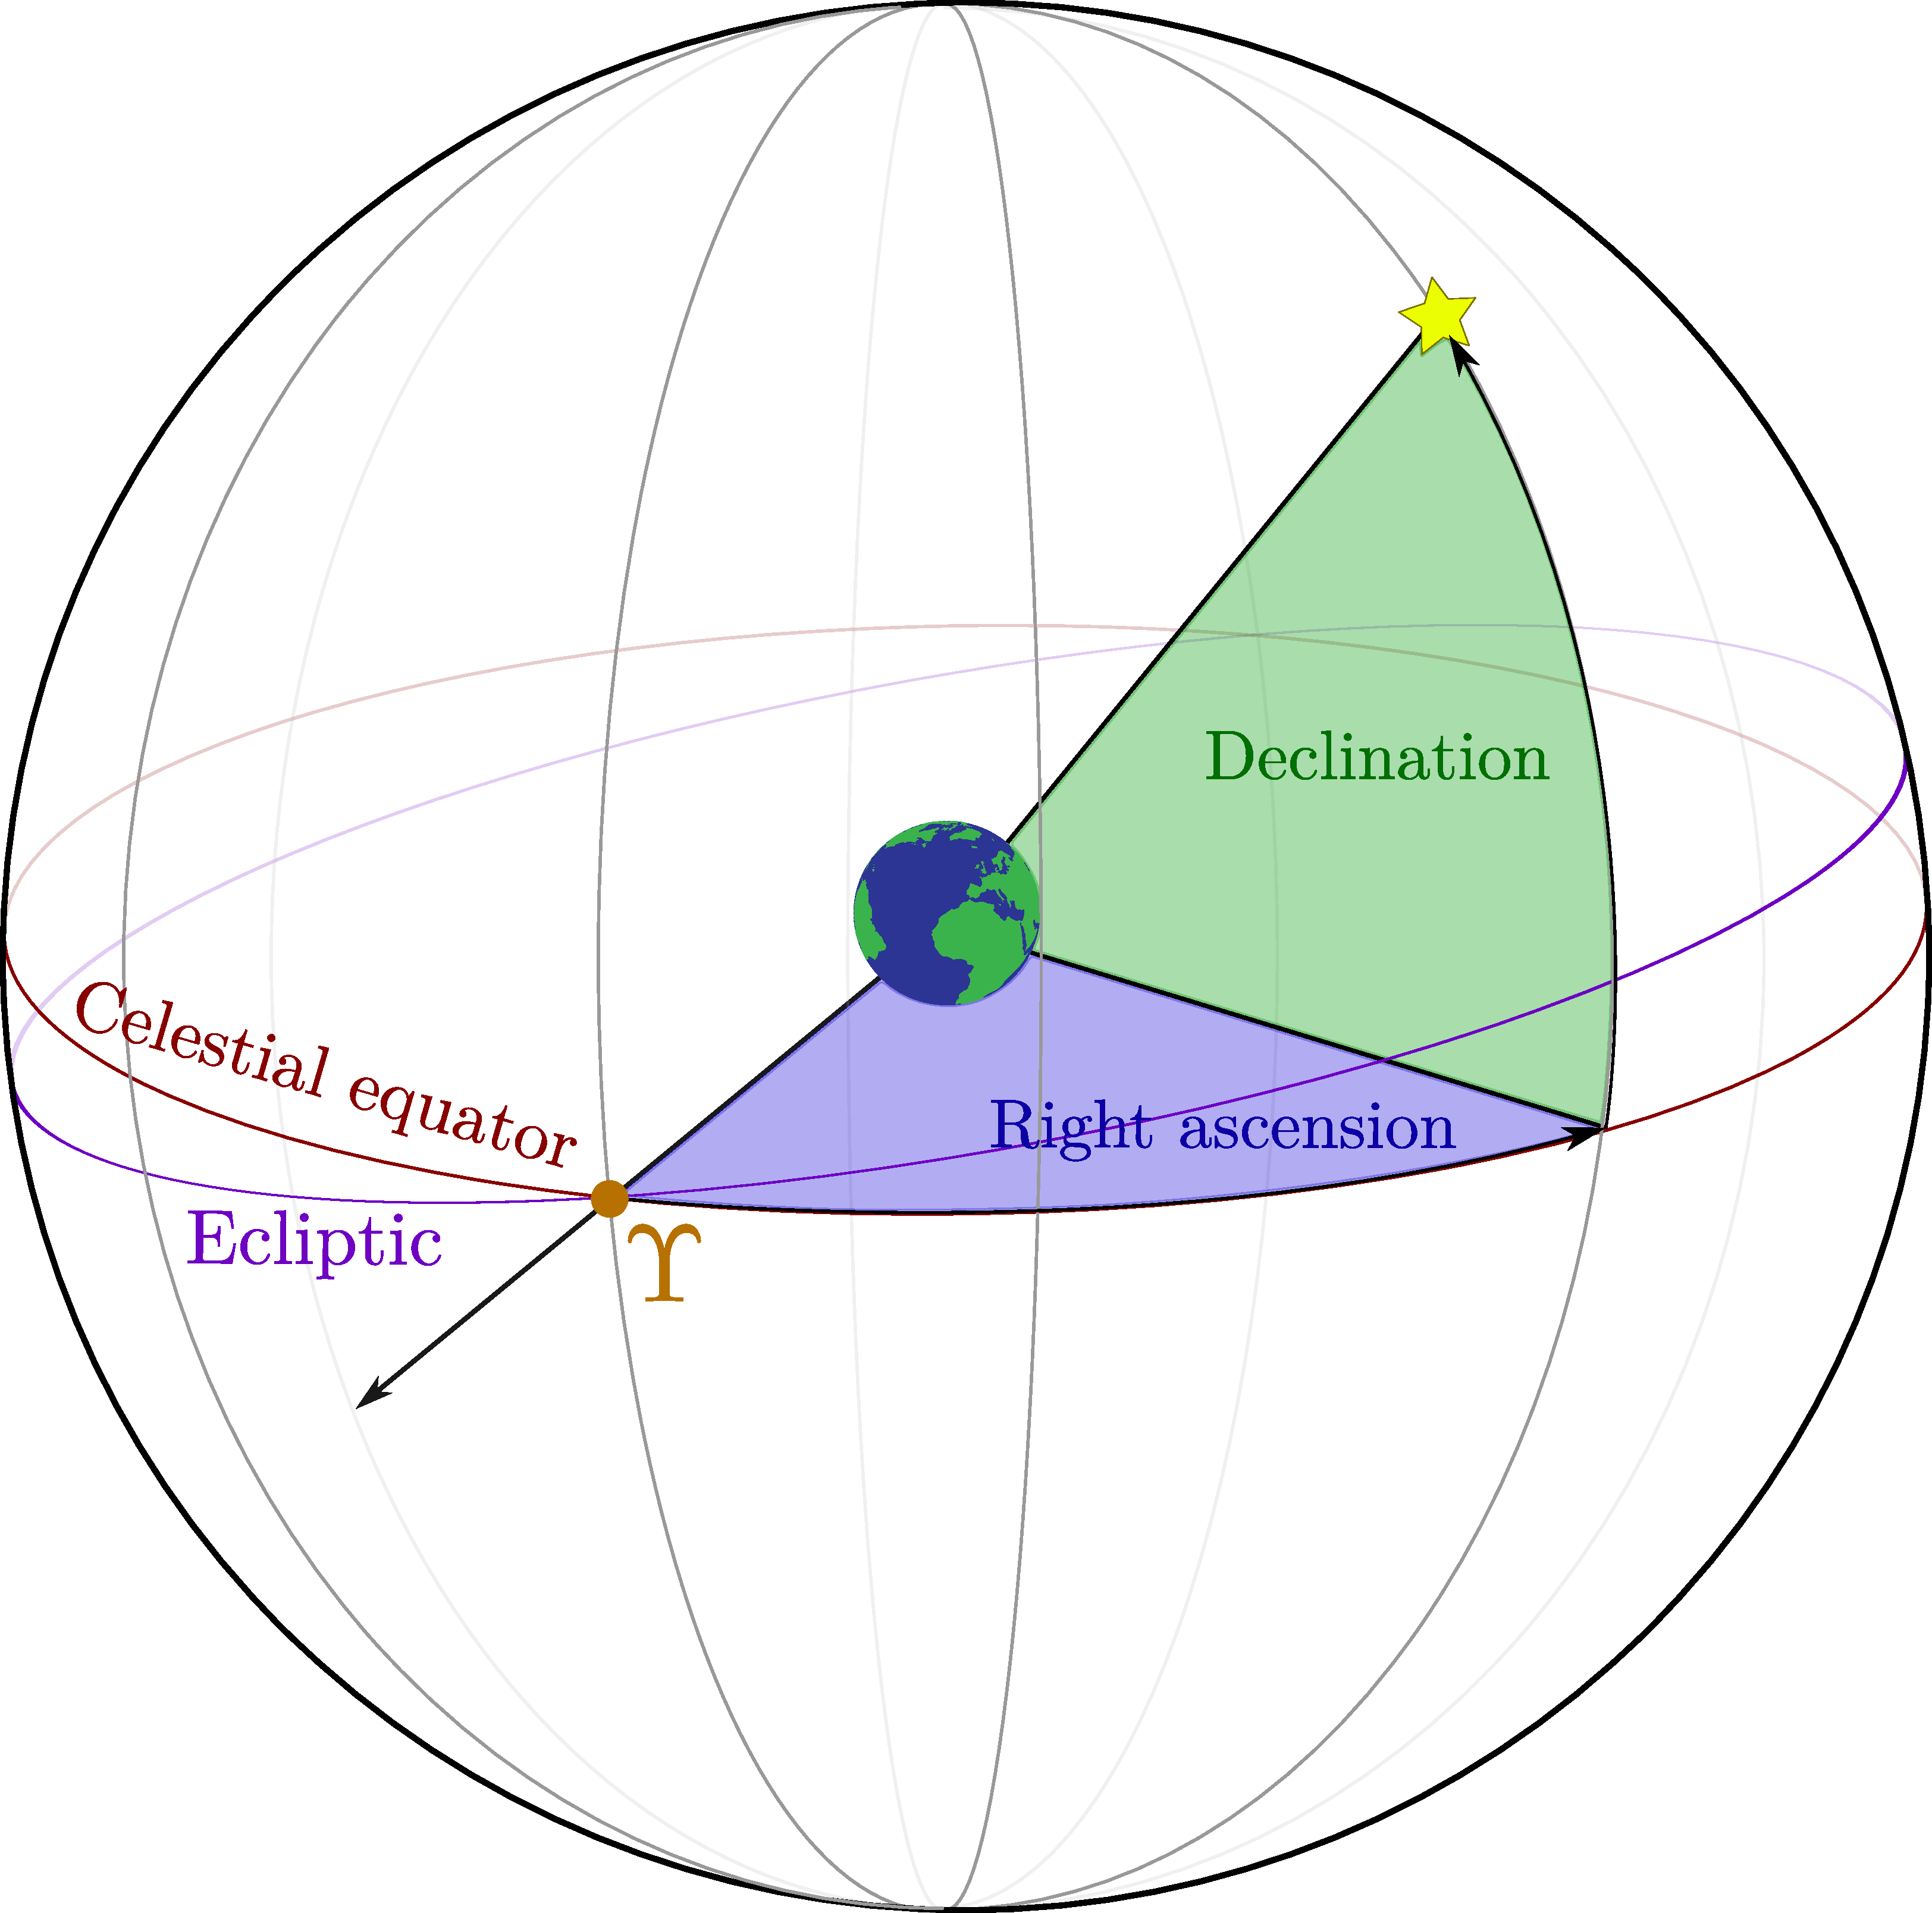
\includegraphics[width=\textwidth]{Images/right_ascension-decli.pdf}
    \caption{Right ascension and declination of a star in the celestial sphere}
    \label{fig:right_ascesion}
  \end{minipage}
  \hspace{0.02\textwidth}
  \begin{minipage}[ht]{0.47\textwidth}
    \centering
    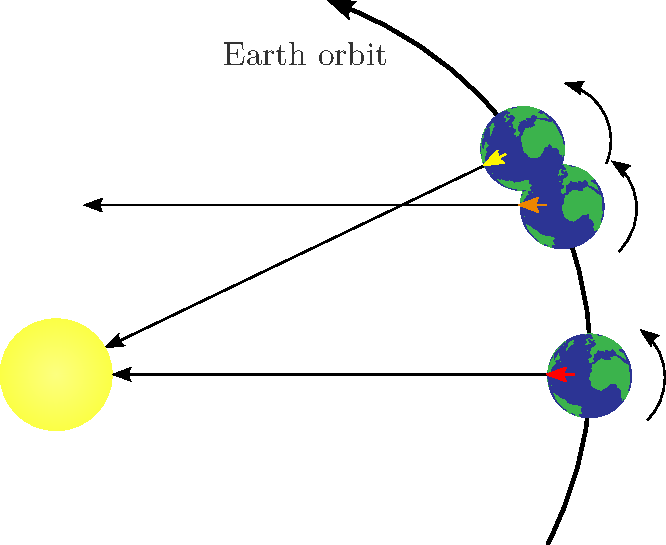
\includegraphics[width=\textwidth]{Images/sidereal.pdf}
    \caption{Graphical representation of the difference between a solar day (yellow) and a sidereal day (orange). (not to scale)}
    \label{fig:sidereal}
  \end{minipage}
\end{figure}
Due to Kepler's second law, the Earth's non-circular orbit around the Sun results in some days being shorter than others. As a result, the actual position of the Sun is not ideal for precise time measurement. The introduction of a \emph{mean Sun} is, thus, a necessity.

\begin{definition}
  The \emph{mean Sun} is a fictitious Sun that moves along the celestial equator at a constant rate \cite{vallado}. This rate is determined in order to make the real Sun and the mean Sun coincide at the vernal equinox. We define the \emph{mean solar time} as the hour angle (along the celestial equator) between the local meridian and the meridian of the mean Sun.
\end{definition}
It is worth noting that unlike the real Sun, the mean Sun moves along the celestial equator, rather than the ecliptic.
\begin{definition}
  We define the \emph{prime meridian} or \emph{zero meridian} as the meridian on the celestial sphere that passes through the Royal Observatory in Greenwich, England (when projected on the Earth).
\end{definition}
\begin{definition}
  The \emph{Greenwich Mean Time} (GMT) or \emph{Universal Time} (UT) is the hour angle of the mean Sun measured from the prime meridian and counted from midnight. That is, when the prime meridian and mean Sun meridians coincide, the GMT is 12:00.
\end{definition}
The use of two distinct names, namely GMT and UT, to refer to the same time can be attributed to historical reasons. Initially, GMT was defined as the mean solar time at the prime meridian with 00:00 GMT coinciding with the moment when the mean Sun was at the that meridian. On the other hand, UT was introduced as a 12-hour translation of GMT, intended for civilian purposes. Eventually, GMT was redefined to align with UT.

In the middle of the 20th century, \emph{Ephemeris Time} (ET) was introduced to cope with the irregularities of the Earth's rotation (see \cref{sec:reference_systems}). This time was defined from historical observations of planets in a Newtonian physics framework, isolating the time from the equations, and the origin of time was chosen coherently with GMT, at January 0, 1900, 12:00 GMT (JD 2415020.0). This timescale provided a uniform time, although it was more difficult to measure than the mean solar time. In the meantime, atomic clocks were invented and at 1967 the \emph{atomic time} (TAI, from French \emph{Temps Athomique International}) was adopted as the SI unit of second. The origin was chosen such that the TAI matched UT at the 00:00:00 UT of January 1st, 1958, and at that time the ET was displaced from UT by 32.184 seconds. At the end of the 20th century, the \emph{Terrestrial Time} (TT) was introduced within a relativistic framework in order to replace ET and provide a smooth and more accurate continuation of it yielding the relation \cite{montenbruck}:
\begin{equation}
  \text{TT}=\text{ET}= \text{TAI} + 32.184\,\mathrm{s}
\end{equation}

For astronomical calculations, it is convenient to consider a timescale defined directly from Earth's rotation, known as \emph{sidereal time}. Namely, \emph{Greenwich Mean Sidereal Time} (GMST) is defined as the angle between the prime meridian and the mean vernal equinox of date (see \cref{sec:reference_systems}). Due to unpredictable irregular changes on the rotation of the Earth, the GMST cannot be computed directly with a formula in terms of the TAI or TT.

The \emph{Universal Time 1} (UT1) is the presently used form of Universal time, and it is defined in terms of Earth's rotation with the following deterministic formula given in \cite{aoki}. For each day, the 00:00 UT1 is defined as the time instant in which GMST has the value:
\begin{equation}
  \mathrm{GMST}(0\text{h UT1})=24110.54841+8640184.812866{T_{\text{UT1},0}}+0.093104{T_{\text{UT1},0}}^2-6.2\cdot 10^{-6}{T_{\text{UT1},0}}^3
\end{equation}
where $T_{\text{UT1},0}=\frac{\text{JD}(0\text{h UT1})-2451545}{36525}$ denotes the number of Julian centuries that have passed since January 2000, 1.5 UT1 at the beginning of the day. The units of the coefficients are seconds. For any instant of time during the day, the following formula is used:
\begin{multline}
  \mathrm{GMST}(\mathrm{UT1})=24110.54841+8640184.812866{T_{\text{UT1}}}+1.002737909350795\cdot240\text{UT1}+\\+0.093104{T_{\text{UT1}}}^2-{6.2\cdot 10^{-6}}{T_{\text{UT1}}}^3
\end{multline}
where $T_\text{UT1}=\frac{\text{JD}(\text{UT1})-2451545}{36525}$ and UT1 are measured in seconds. The coefficient $\omega:=1.002737909350795$ is the Earth's mean angular velocity in degrees per second and the coefficient $240=\frac{3600}{15}$ is the number of seconds in one degree\footnote{Recall that $15^\circ=1\ \text{h}$, $60'=1^\circ$, $60''=1'$, where $''$ are arc seconds and $'$ are arc minutes.}. Similarly to the GMST, there is no simple conversion between the UT1 and the TT or TAI. Instead, IERS\footnote{More information on \href{https://www.iers.org}{https://www.iers.org} (Accessed on June 8, 2023).} (\emph{International Earth Rotation and Reference Systems Service}) provides regularly a bulletin with the difference $\Delta T:= \mathrm{TT}-\mathrm{UT1}$ at several dates. Interpolating these values we can obtain UT1 from TT at any epoch.

Finally, our everyday clock is based on the \emph{Coordinated Universal Time} (UTC). It is defined to be as uniform as the TAI but always kept closer than 0.9 seconds to the UT1 in order to resemble a mean solar time (see \cref{fig:time_graph}). Scientists achieve this by introducing a \emph{leap second} (see \cref{fig:leapsecond}), which is an extra second added to UTC at irregular intervals. \cref{fig:time_graph} summarizes all the time systems introduced in the document.

\begin{figure}[htbp]
  \centering
  \begin{minipage}[ht]{0.45\textwidth}
    \centering
    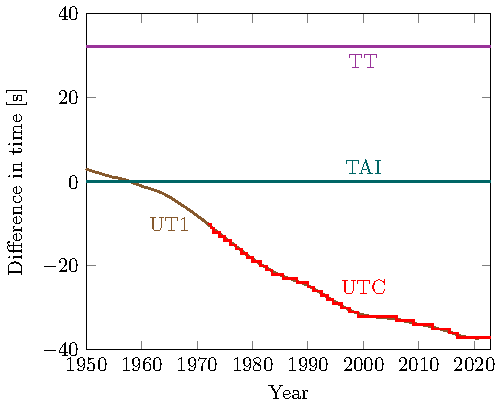
\includegraphics[width=\textwidth]{Images/time_graph.pdf}
    \caption{Evolution of times TT, UT1 and UTC in comparison with TAI. \cite{iersDeltaT}}
    \label{fig:time_graph}
  \end{minipage}
  \hspace{0.0333333\textwidth}
  \begin{minipage}[ht]{0.45\textwidth}
    \centering
    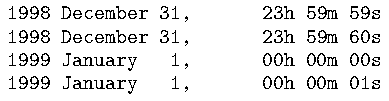
\includegraphics[width=0.9\textwidth]{Images/leap_second.pdf}
    \caption{Leap second introduced to the UTC time at the end of the December 1998. \cite{iersbulletinC}}
    \label{fig:leapsecond}
  \end{minipage}
\end{figure}

We summarize here useful conversions between time systems:
\begin{align*}
  \begin{split}
    \mathrm{GMST}(\mathrm{UT1})&=24110.54841+8640184.812866{T_{\text{UT1}}}+1.002737909350795\cdot240\text{UT1}+\\
    &\hspace{8cm}+0.093104{T_{\text{UT1}}}^2-{6.2\cdot 10^{-6}}{T_{\text{UT1}}}^3
  \end{split} \\
  \text{UT1} & =\text{TT}-\Delta T                                                                                         \\
  \text{TT}  & =\text{TAI}-32.184                                                                                          \\
  \text{TAI} & =\text{UTC}+\delta
\end{align*}
where $\Delta T$ is the difference between the TT and UT1, and $\delta$ is a piecewise constant function that counts the number of leap seconds introduced since 1972, when they were introduced for the first time. All the numbers have units of second. Note that since the rotation of the Earth cannot be predicted accurately, $\Delta T$ can only be determined retrospectively, and is given by the \emph{International Earth Rotation and Reference Systems Service} (IERS).
\subsubsection{Reference systems}\label{sec:reference_systems}
It is well-known that Newton's second law is only valid when applied to an \emph{inertial reference frame}, that is, a frame of reference that is not undergoing any acceleration. In practice, however, almost any frame of reference is non-inertial. So in this chapter we will describe a quasi-inertial frame of reference which will be used to integrate Newton's second law. On the other hand, since the Earth is not a body with a homogeneous density of mass, there are zones with higher mass density than others, and therefore with higher gravitational pull (see \cref{sec:laplace_spherical_potential}). Therefore, we will need the longitude and latitude of the satellite with respect to the Earth at each time of integration in order to place it in the correct position with respect to the Earth.

Based on our study of satellite motion around the Earth, it is natural to place all the origins of the reference frames considered throughout the document at the center of mass of the Earth.

The first reference frame we must consider is the \emph{celestial} one. In the celestial frame, the $x$-axis is defined as the line of intersection between the equatorial plane and the ecliptic plane. The positive direction is chosen to point towards the vernal equinox. The $z$-axis is chosen to be perpendicular to the equatorial plane and the $y$-axis is such that the triplet $(x,y,z)$ is a right-handed system.

However, due to the presence of other solar system planets (and other smaller perturbations), the orbital plane of the Earth is not fixed in space, but is subjected to a small variation called \emph{planetary precession}. Moreover, the gravitational attraction of the Sun and Moon on the Earth's equator cause Earth's axis of rotation to precess similarly to the action of a spinning top with a period of about 26000 years \cite{montenbruck}. This motion is called \emph{lunisolar precession}. On the other hand, smaller perturbations in amplitude and shorter period (around $<18.6$ years \cite{wiki:eci}) superposed with the precessional motion creates a motion called \emph{nutation}. When this latter oscillations are averaged out, the vernal equinox and the equator are referred to \emph{mean} values, rather than \emph{true} values.

In addition, the Earth's axis of rotation undergoes a slight periodic motion around a reference axis of rotation, that passes through the \emph{IRP} (\emph{IERS Reference Pole}). This motion is called \emph{polar motion} and is caused by the redistribution of the Earth's mass due to the seasonal variations of the atmosphere and the oceans. The polar motion is usually described by the \emph{CEP} (\emph{Celestial Ephemeris Pole}), which is the intersection of the Earth's axis of rotation with the celestial sphere. In \cref{fig:prec_nut} we summarize the different types of perturbations on the Earth's axis of rotation.

\begin{figure}[ht]
  \centering
  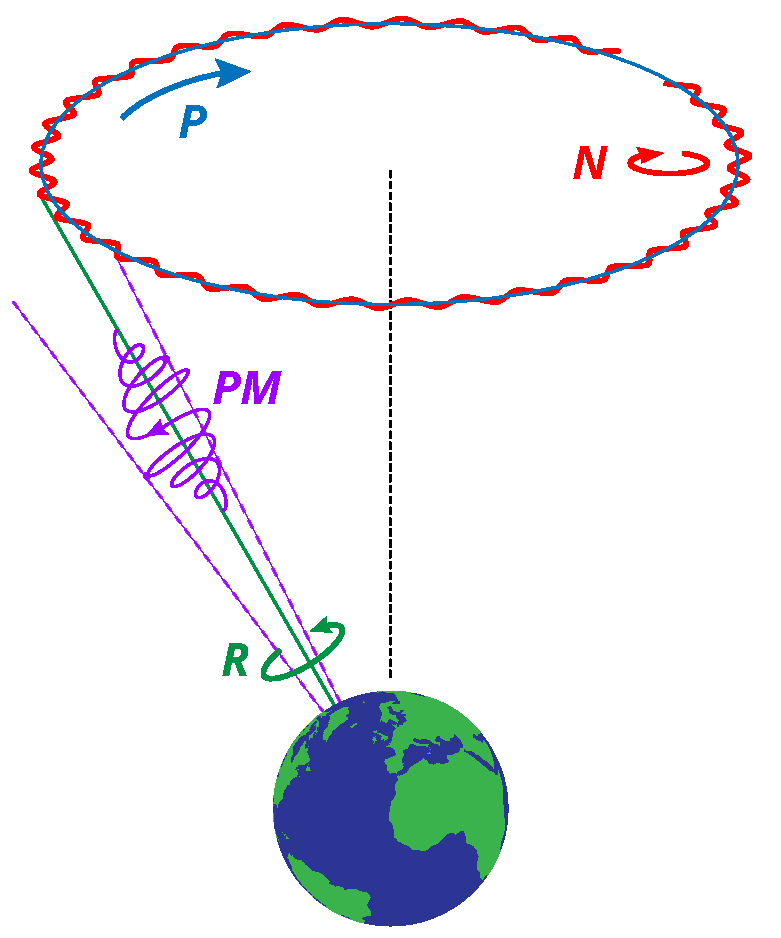
\includegraphics[width=0.5\textwidth]{Images/precession_nutation.pdf}
  \caption{Graphical explanation of the perturbation by precession (blue), nutation (red) and polar motion (violet) of the Earth's axis of rotation (green).}
  \label{fig:prec_nut}
\end{figure}

In view of this time-dependent orientation of both the ecliptic and the equator, the standard-reference frame chosen is based on the mean equator, ecliptic and mean equinox of a fixed time, the beginning of the year 2000, namely at 12:00 TT on 1st January 2000, the so-called \emph{J2000 epoch}.
\begin{definition}[Earth-centered inertial frame]
  We define the \emph{J2000 reference frame} as the reference frame whose $x$-axis is the intersection of the mean celestial equator and the ecliptic of the J2000 epoch, pointing at the mean vernal equinox of the same epoch; the $z$-axis is perpendicular to the mean equator, and the $y$-axis is chosen such that the triplet $(x,y,z)$ is a right-handed system. This frame of reference is also called \emph{Earth-centered inertial} (ECI) frame.
\end{definition}

Let's introduce now an Earth-fixed reference frame.
\begin{definition}[Earth-centered, Earth-fixed frame]
  We define the \emph{Earth-centered, Earth-fixed frame of reference} (ECEF) as the frame of reference whose $x$-axis is pointing to the prime meridian, the $z$-axis is perpendicular to the Earth's equator and the $y$-axis is chosen such that the triplet $(x,y,z)$ is a right-handed system.
\end{definition}
These two coordinate systems have, as mentioned earlier, the origin at the center of mass of the Earth. Note that, the ECEF frame is not inertial, since it is rotating with the Earth.
\subsubsection{Conversion between reference systems}

As we noted in the previous section the angle $\varepsilon$ between the celestial equator and ecliptic planes is not constant due to the planetary precession.

Our goal in this section is to transform the position of the satellite from the ECI system to the ECEF system and vice versa. This rotation transformation is given by a product of 4 rotations matrices:
\begin{itemize}
  \item the precession matrix $\vf{P}$,
  \item the nutation matrix $\vf{N}$,
  \item the Earth rotation matrix $\vf\Theta$, and
  \item the polar motion matrix $\vf\Pi$.
\end{itemize}
These matrices are such that:
\begin{equation}
  \vf{r}_\mathrm{ECEF}(t)=\vf\Pi(t)\vf\Theta(t)\vf{N}(t)\vf{P}(t)\vf{r}_\mathrm{ECI}(t)
\end{equation}
where $\vf{r}_\mathrm{ECEF}(t)$ is the position vector of the satellite in the ECEF frame at time $t$ and $\vf{r}_\mathrm{ECI}(t)$ is the position vector of the satellite in the ECI frame at time $t$. From here on, we will omit the evaluation on the time $t$ for the sake of simplicity. Let's now argue why the transformation has this particular form.

The precession matrix is responsible for \emph{eliminating} all the movement due to the planetary and lunisolar precession. Thus, $\vf{P}$ transforms the mean equator and mean equinox at time J2000 to the respective values at time $t$. With the help of \cref{fig:precession_matrix}, one can check that this transformation is given by:
\begin{equation}
  \vf{P}=\vf{R}_z(-90-z)\vf{R}_x(\theta)\vf{R}_z(90-\zeta)
\end{equation}
And with a bit of algebra it can be simplified to:
\begin{equation}
  \vf{P}=\vf{R}_z(-z)\vf{R}_y(\theta)\vf{R}_z(-\zeta)
\end{equation}
Recall that the fundamental rotation matrices $\vf{R}_x(\theta)$, $\vf{R}_y(\theta)$ and $\vf{R}_z(\theta)$ are with respect to the axis of the J2000 frame, and they are given by:
\begin{equation}
  \vf{R}_x(\varphi)=\begin{pmatrix}
    1 & 0            & 0           \\
    0 & \cos\varphi  & \sin\varphi \\
    0 & -\sin\varphi & \cos\varphi
  \end{pmatrix}\;\;\;
  \vf{R}_y(\varphi)=\begin{pmatrix}
    \cos\varphi & 0 & -\sin\varphi \\
    0           & 1 & 0            \\
    \sin\varphi & 0 & \cos\varphi
  \end{pmatrix}\;\;\;
  \vf{R}_z(\varphi)=\begin{pmatrix}
    \cos\varphi  & \sin\varphi & 0 \\
    -\sin\varphi & \cos\varphi & 0 \\
    0            & 0           & 1
  \end{pmatrix}
\end{equation}
where we have used the convention of signs given by \cite{goldstein}.
\begin{figure}[htbp]
  \centering
  \begin{minipage}[ht]{0.45\textwidth}
    \centering
    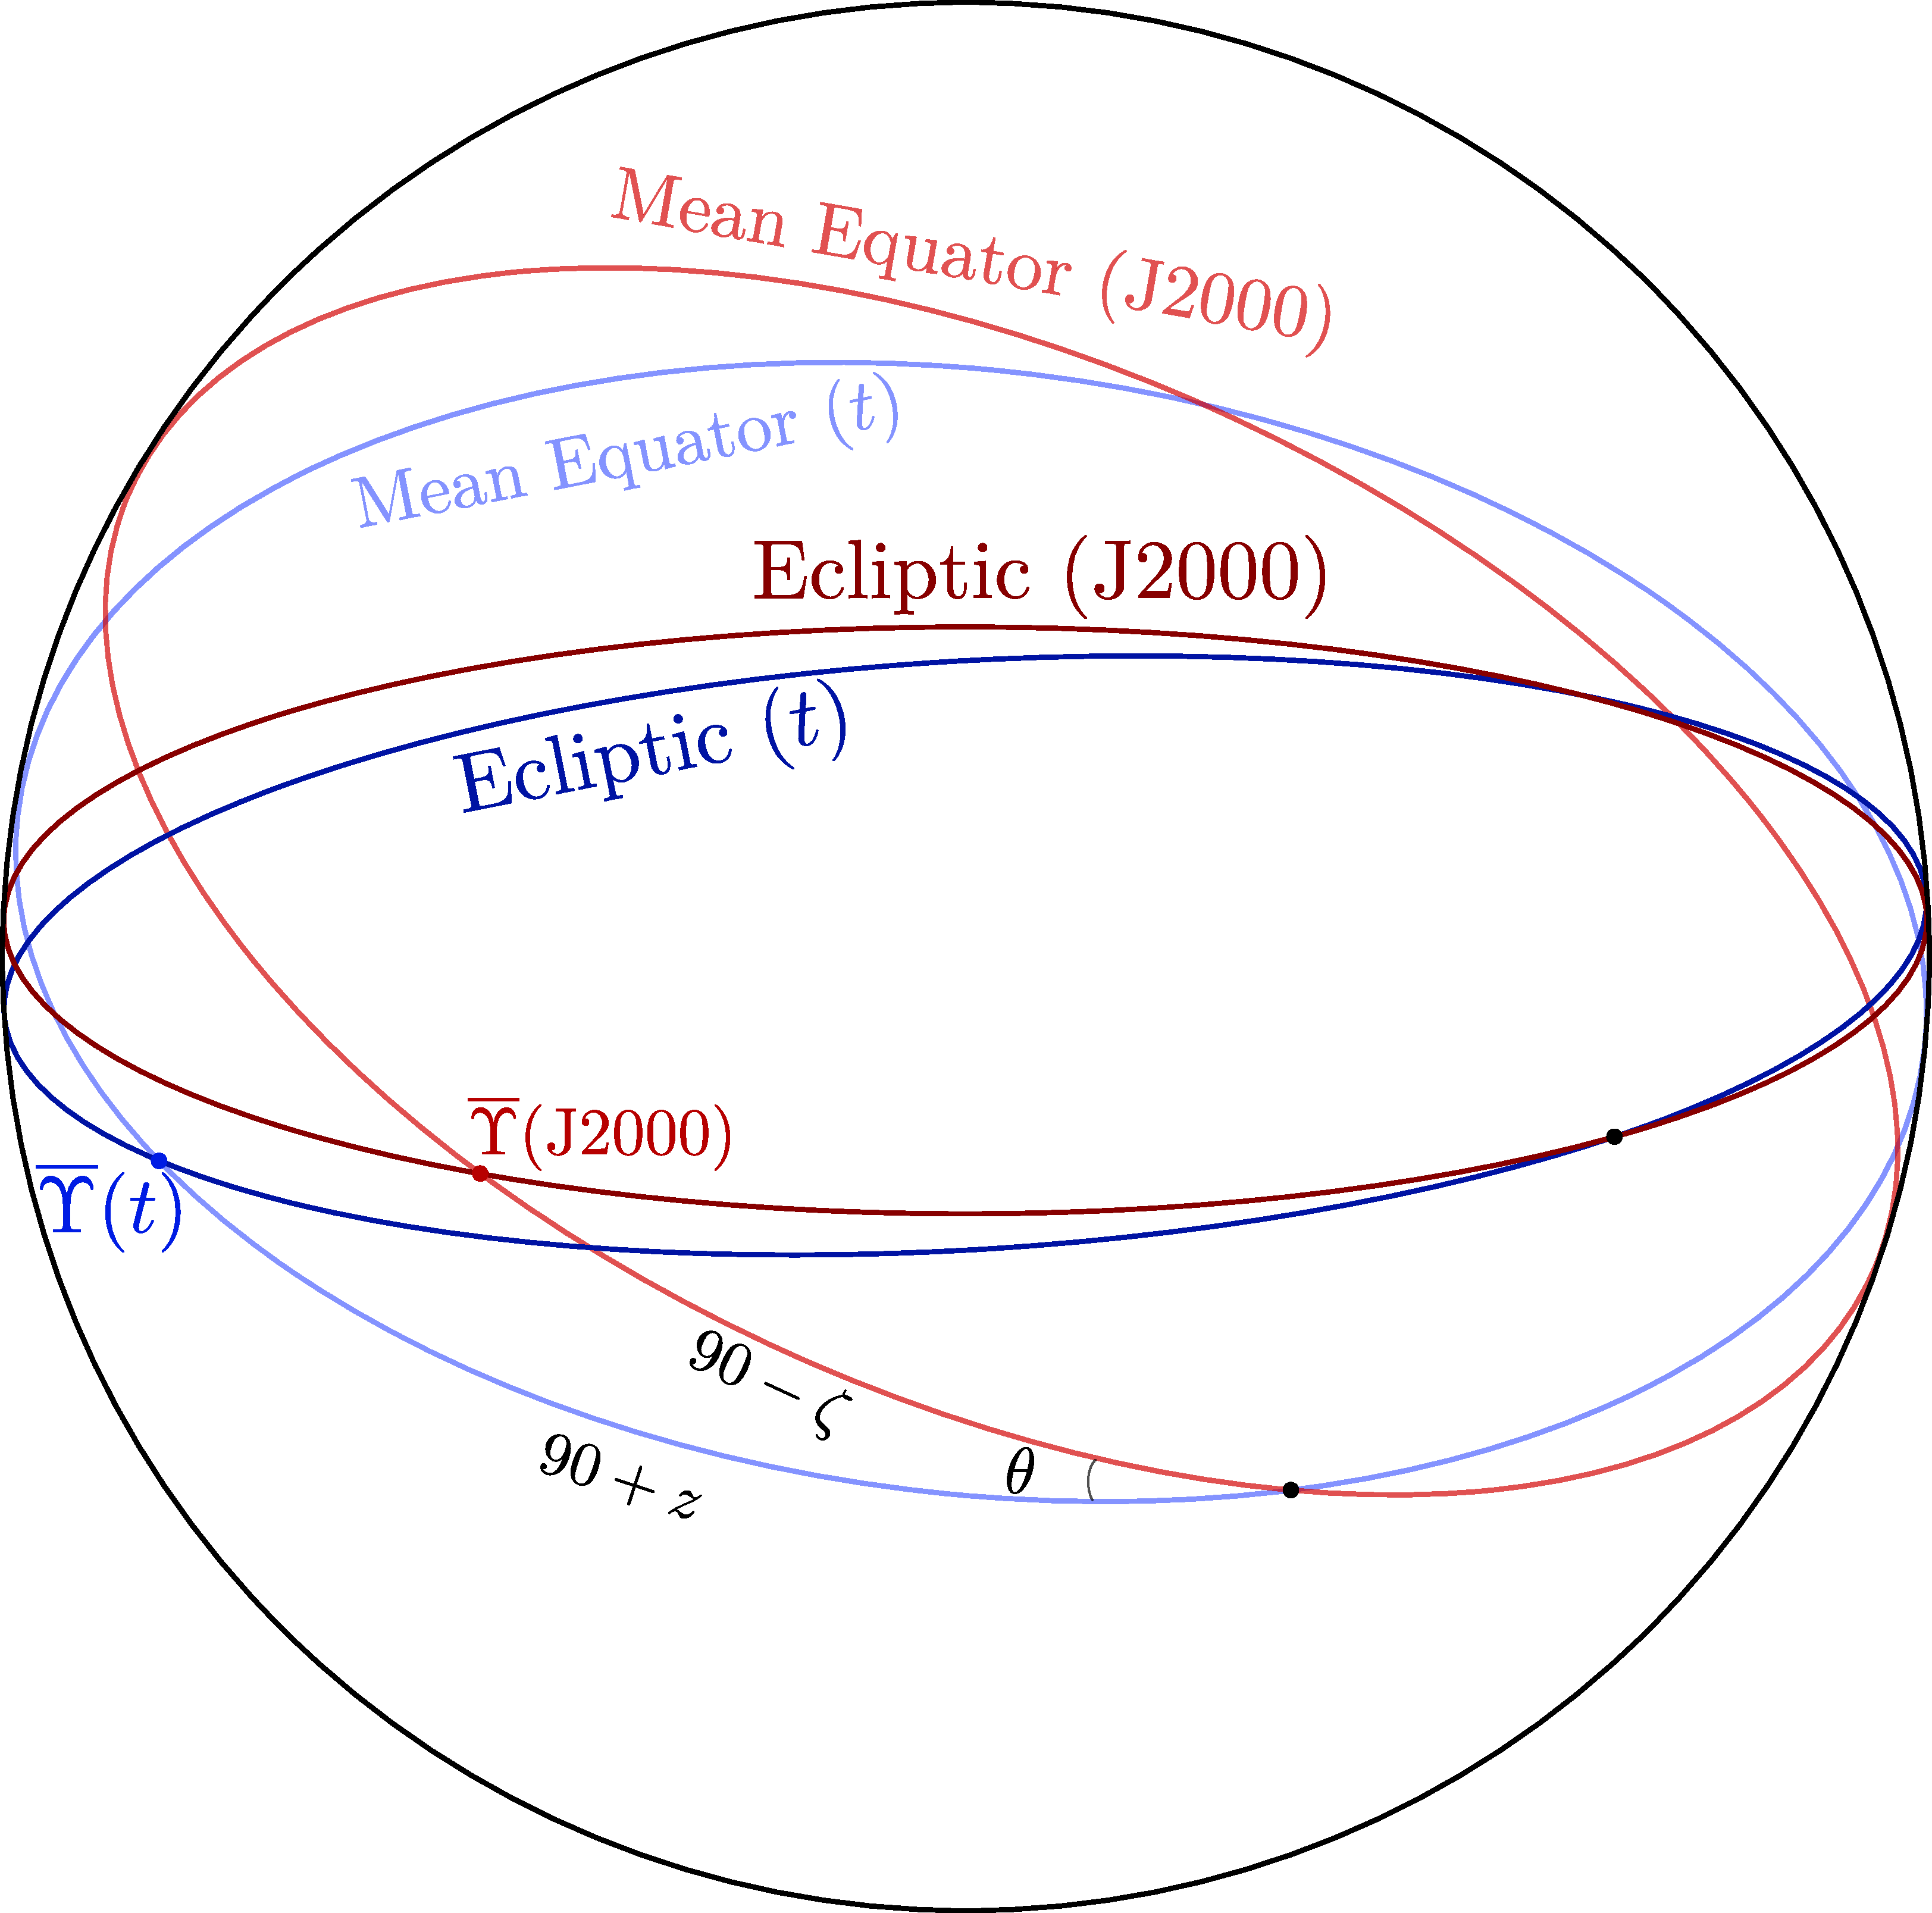
\includegraphics[width=\textwidth]{Images/ecliptic_equator.pdf}
    \caption{Celestial sphere showing the ecliptic and the equator of both the epoch J2000 and the current epoch $t$. Dark colors represent the ecliptic while light colors represent the equator. On the other hand, red colors represents the J2000 epoch and blue colors represents the current epoch $t$. Source: based on \cite{montenbruck}.}
    \label{fig:precession_matrix}
  \end{minipage}
  \hspace{0.0333333\textwidth}
  \begin{minipage}[ht]{0.45\textwidth}
    \centering
    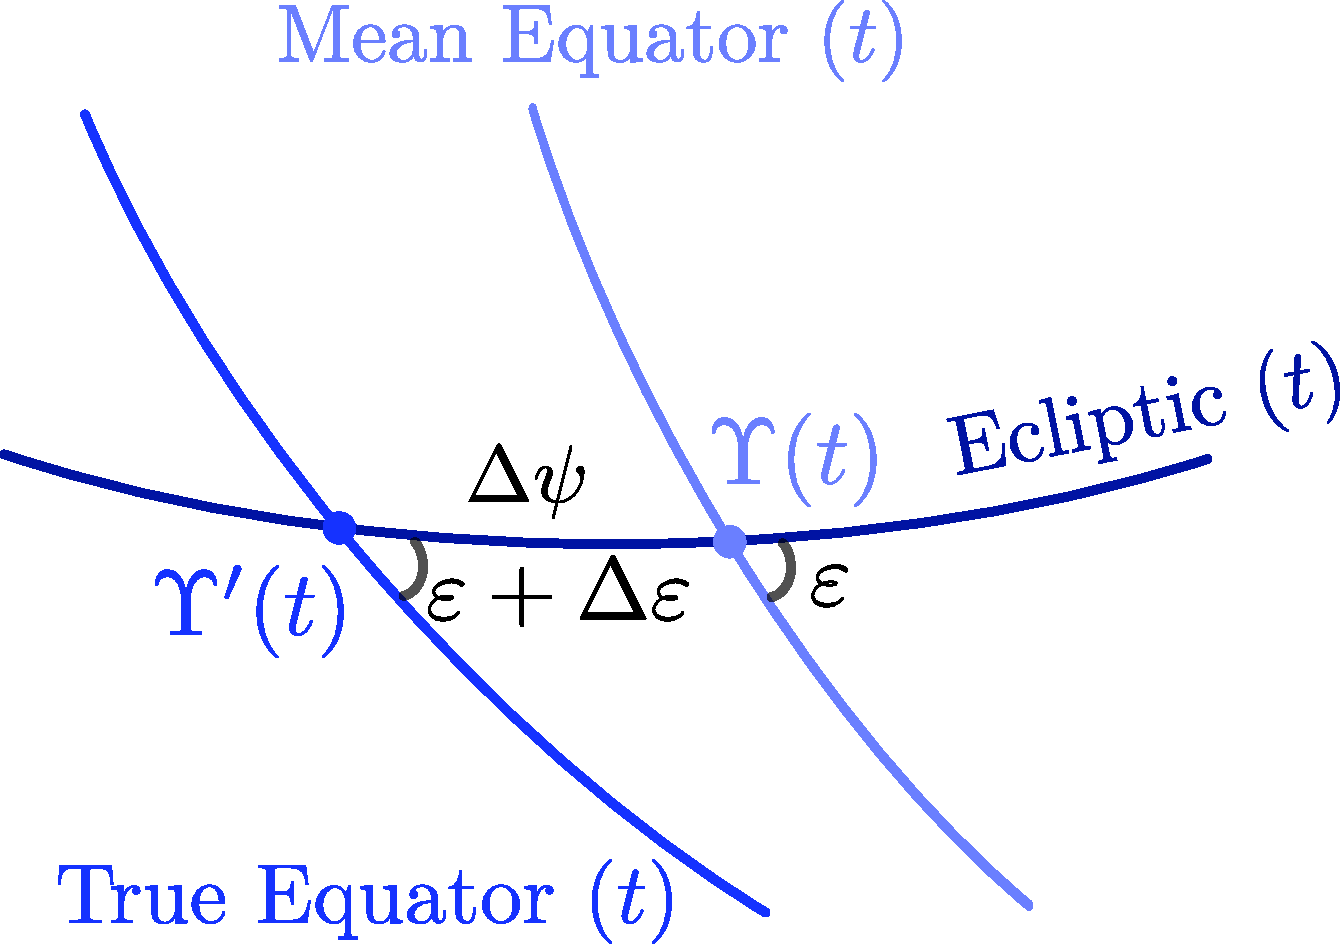
\includegraphics[width=\textwidth]{Images/nutation_matrix.pdf}
    \caption{True equator and mean equator, and true equinox ($\Upsilon$) and mean equinox ($\overline\Upsilon$) at a given epoch $t$ together with the ecliptic at that time. Source: based on \cite{montenbruck}.}
    \label{fig:nutation_matrix}
  \end{minipage}
\end{figure}
The reader may wonder why we have used the notation $90-z$ and $90-\zeta$ instead of $z$ and $\zeta$ (for example) for the angles in question. The reason is related to the precise definition of these angles from the pole of the celestial sphere rather than from where we have defined them, but we will not elaborate on this point here. Nonetheless, we have chosen this notation to maintain consistency with related articles \cite{lieske}.

The nutation perturbations are removed by the nutation matrix $\mathbf{N}$. This matrix transforms the coordinates of the mean equator and equinox at epoch $t$ to those of the true equator and equinox at the same epoch, respectively. Hence, from figure \cref{fig:nutation_matrix} we can see that the nutation matrix is given by:
\begin{equation}
  \mathbf{N}=\vf{R}_x(-\varepsilon-\Delta \varepsilon)\vf{R}_z(-\Delta \psi)\vf{R}_x(\varepsilon)
\end{equation}

In \cref{sec:time_measurement} we defined the GMST as the hour angle between the mean vernal equinox and the prime meridian, measured on the true equator. Similarly, we define the \emph{Greenwich Apparent Sidereal Time} (GAST) as the hour angle between the true vernal equinox and the prime meridian, measured on the true equator too. The difference between these two times is given by the so-called \emph{equation of the equinoxes}, which up to first order in the nutation angles is given by (see \cref{fig:nutation_matrix}):
\begin{equation}
  \text{GAST}- \text{GMST}\simeq\Delta \psi\cos(\varepsilon+\Delta \varepsilon)
\end{equation}
The Earth rotation matrix $\vf{\Theta}$ is responsible for aligning satellite with his actual meridian at the time of the observation. This matrix is given by:
\begin{equation}
  \vf\Theta=\vf{R}_z(\text{GAST})
\end{equation}
Finally the polar motion movement around the CEP axis is modelled with the matrix $\vf\Pi$ given by:
\begin{equation}
  \vf\Pi=\vf{R}_y(- x_p)\vf{R}_x(- y_p)
\end{equation}

\begin{figure}[htbp]
  \centering
  \begin{minipage}[ht]{0.45\textwidth}
    \centering
    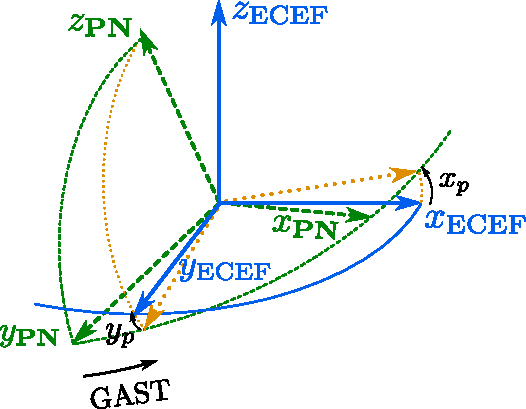
\includegraphics[width=\textwidth]{Images/polar_motion_matrix.pdf}
    \caption{Three reference frames used to transform from the ECI frame to the ECEF frame. In green, the ECI frame once applied the precession and nutation transformations. In orange, the transformation of the green system once applied the rotation matrix $\vf\Theta$. Finally, in blue, the transformation of the orange system once applied the polar motion matrix $\vf\Pi$.}
    \label{fig:polar_motion_matrix}
  \end{minipage}
  \hspace{0.0333333\textwidth}
  \begin{minipage}[ht]{0.45\textwidth}
    \centering
    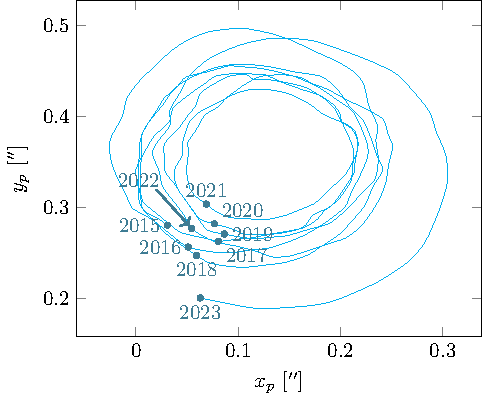
\includegraphics[width=\textwidth]{Images/polar_motion.pdf}
    \caption{Graphical representation of evolution of the CEP with respect to IRP (placed at the origin of the graphic) due to polar motion. The blue dots indicate the position of the CEP at the beginning of the respective years. Data from \cite{eop}.}
    \label{fig:polar_motion}
  \end{minipage}
\end{figure}

In \cref{fig:polar_motion_matrix} we can see a graphical representation of these two latter transformation matrices. The parameters $x_p$ and $y_p$ are constantly updated in the IERS bulletins \cite{iersbulletinA}. All the other parameters are given in \cite{lieske}, and we provide here a summary of them:
\begin{align}
  \varepsilon & = 23.4392911^\circ -46.8150''T - 0.00059''T^2 + 0.001813''T^3 \\
  \zeta       & = 2306.2181''+ 0.30188''T + 0.017998''T^2                     \\
  \theta      & = 2004.3109''T- 0.42665''T^2 - 0.041833''T^3                  \\
  z           & = 2306.2181'' + 1.09468''T^2+0.018203''T^2
\end{align}
where $T=\frac{\text{JD}_{TT} - 2451545}{36525}$ are the Julian centuries that have elapsed since the J2000 epoch. The values for nutations $\Delta \psi$ and $\Delta \varepsilon$ can be expanded into \cite{montenbruck}:
\begin{equation}
  \Delta\psi = \sum_{i=1}^{106} {(\Delta\psi)}_i\sin \phi_i\qquad \Delta\varepsilon = \sum_{i=1}^{106} {(\Delta\varepsilon)}_i\cos \phi_i
\end{equation}
where $\phi_i=p_{\ell,i}\ell+ p_{\ell',i}\ell'+p_{F,i}F+p_{D,i}D+p_{\Omega,i}\Omega$, $p_{\ell,i}$, $p_{\ell',i}$, $p_{F,i}$, $p_{D,i}$, $p_{\Omega,i}$ are integer coefficients and the other variables are the Moon's mean anomaly ($\ell$), the Sun's mean anomaly $(\ell')$, the mean distance of the Moon from the ascending node ($F$), the difference between the mean longitudes of the Sun and the Moon ($D$), and the mean longitude of the ascending node of the Moon ($\Omega$). We will not go into detail about these variables, there are explicit expressions for them in \cite{montenbruck} as a function of $T=\frac{\text{JD}_{TT} - 2451545}{36525}$:
\begin{align}
  \ell   & = 134^\circ 57' 46.733'' + 477198^\circ 52' 02.633'' T + 31.310'' T^2 + 0.064'' T^3 \\
  \ell'  & = 357^\circ 31' 39.804'' + 35999^\circ 03'01.224'' T - 0.577'' T^2 - 0.012'' T^3    \\
  F      & = 93^\circ 16' 18.877'' + 483202^\circ 01' 03.137'' T - 13.257'' T^2 - 0.011'' T^3  \\
  D      & = 297^\circ 51' 01.307'' + 445267^\circ 06' 41.328'' T - 6.891'' T^2 + 0.019'' T^3  \\
  \Omega & = 125^\circ 02' 40.280'' - 1934^\circ 08' 10.539'' T + 7.455'' T^2 + 0.008'' T^3
\end{align}

Some of these integer coefficients together with the values of the amplitudes ${(\Delta\psi)}_i$ and ${(\Delta\varepsilon)}_i$  are given in \cref{tab:nutation_coefficients}.
\begin{table}[ht]
  \centering
  \begin{tabular}{|c|ccccc|c|c|}
    \hline
    $i$    & $p_{\ell,i}$ & $p_{\ell',i}$ & $p_{F,i}$ & $p_{D,i}$ & $p_{\Omega,i}$ & ${(\Delta\psi)}_i\ [0.0001'']$ & ${(\Delta\varepsilon)}_i\ [0.0001'']$ \\
    \hline
    1      & 0            & 0             & 0         & 0         & 1              & $-171996 -174.2T$              & $92025+8.9T$                          \\
    2      & 0            & 0             & 0         & 0         & 2              & $2062+0.2T$                    & $-895+0.5T$                           \\
    3      & $-2$         & 0             & 2         & 0         & 1              & 46                             & $-24$                                 \\
    4      & 2            & 0             & $-2$      & 0         & 0              & $11$                           & 0                                     \\
    5      & $-2$         & 0             & 2         & 0         & 2              & $-3$                           & 1                                     \\
    6      & 1            & $-1$          & 0         & $-1$      & 0              & $-3$                           & 0                                     \\
    7      & 0            & $-2$          & 2         & $-2$      & 1              & $-2$                           & 1                                     \\
    8      & 2            & 0             & $-2$      & 0         & 1              & $1$                            & $0$                                   \\
    9      & 0            & 0             & 2         & $-2$      & 2              & $-13187-1.6T$                  & $5736-3.1T$                           \\
    \vdots & \vdots       & \vdots        & \vdots    & \vdots    & \vdots         & \vdots                         & \vdots                                \\
  \end{tabular}
  \caption{First nutation coefficients \cite{montenbruck}}
  \label{tab:nutation_coefficients}
\end{table}
\subsection{Keplerian orbital elements}
In this section we will introduce the Keplerian orbital elements, which are a set of variables that completely determine the orbit of a satellite and, therefore, they are very useful in the storage of the orbital information of a satellite.
\subsubsection{Keplerian orbital elements from position and velocity}
We first give some preliminary definitions.
\begin{definition}
  Consider a satellite orbiting the Earth. The \emph{orbital plane} is the plane that contains the orbit of the satellite. The \emph{line of nodes} is the line of intersection between the orbital plane and the equatorial plane. Finally, the \emph{ascending node} is the point on the line of nodes and the orbit of the satellite where the satellite crosses the equatorial plane from south to north.
\end{definition}
\begin{definition}[Orbital elements]
  The \emph{Keplerian orbital elements} of a satellite are five independent quantities that completely determine its orbit. If moreover the exact position of the satellite on the orbit is wanted, a sixth quantity is needed. The first five orbital elements are:
  \begin{enumerate}
    \item The \emph{semi-major axis} $a$ of the orbit.
    \item The \emph{eccentricity} $e$ of the orbit.
    \item The \emph{inclination} $i$, which is the angle between the equatorial plane and the orbital plane.
    \item The \emph{longitude of the ascending node} $\Omega$, which is the angle between the vernal equinox and the ascending node.
    \item The \emph{argument of perigee} $\omega$, which is the angle between the ascending node and the periapsis, measured along the orbit.
  \end{enumerate}
  The sixth quantity is the \emph{true anomaly} $\nu$, which is the angle between the periapsis and the position of the satellite on the orbit.
\end{definition}
\begin{figure}[ht]
  \centering
  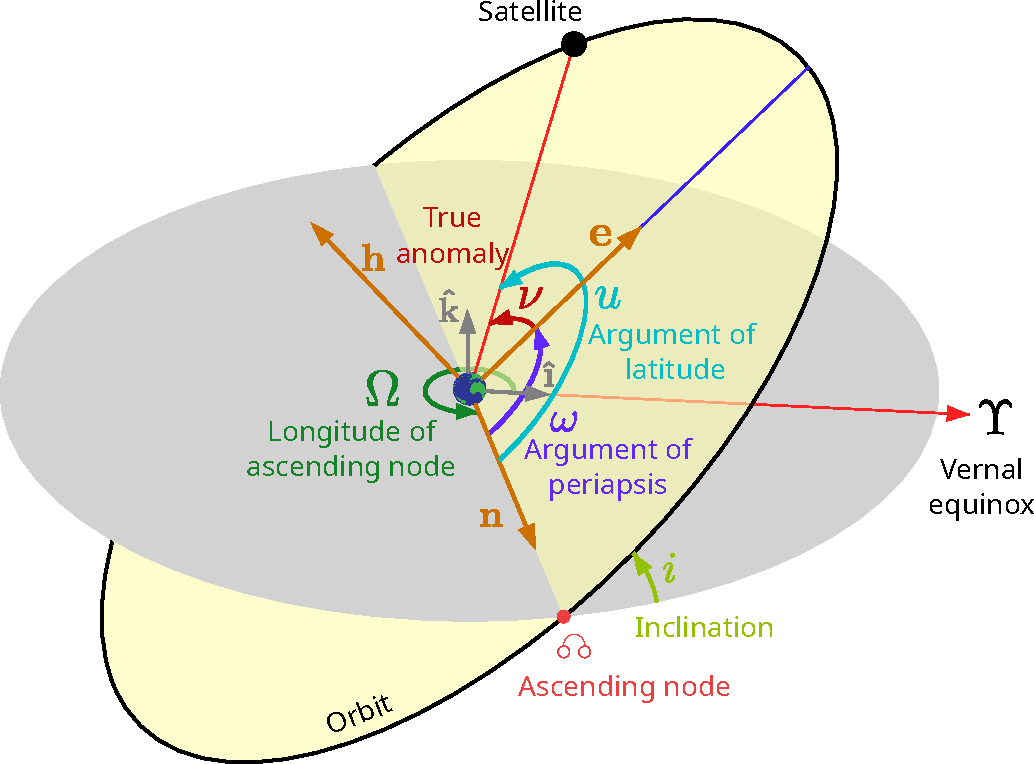
\includegraphics[width=0.8\textwidth]{Images/orbital_elements.pdf}
  \caption{Orbital elements of a satellite. Source: based on \cite{wiki:orbital-elements}.}
  \label{fig:orbital_elements}
\end{figure}
\cref{fig:orbital_elements} shows a schematic representation of these elements. The elements $a$, $e$ and $i$ are always well-defined. However, the elements $\Omega$, $\omega$ and $\nu$ are not always well-defined, namely for $e=0$ or $i=0$. We discuss this in more detail below. For the moment assume $e\neq 0$ and $i\neq 0$. In order to express these elements in terms of the position and velocity of the satellite, we need to introduce the following vectors:
\begin{definition}
  Let $\vf{e}_z=(0,0,1)$ be the unit vector perpendicular to the equatorial plane. We define the vector $\vf{n}:=\vf{e}_z\times \vf{h}$ and the \emph{eccentricity vector} $\vf{e}$ as $\vf{e}:=\vf{B}/\mu$, whose norm is the eccentricity $e$.
\end{definition}
Note that $\vf{n}\perp \vf{e}_z$ and $\vf{n}\perp \vf{h}$ which imply that $\vf{n}$ must lie on the orbital plane and equatorial plane, and therefore, in the line of nodes pointing towards the ascending node, by the right-hand rule. On the other hand, since $\vf{B}$ points towards the periapsis, so does $\vf{e}$. From here, let's obtain the orbital elements in terms of $\vf{r}$ and $\dot{\vf{r}}$.

First, we calculate $\vf{h}=\vf{r}\times\dot{\vf{r}}$ and from here note that the vectors $\vf{n}$ and $\vf{B}$ can be computed directly from $\vf{r}$, $\dot{\vf{r}}$ and $\vf{h}$. Thus, we can get $e$ by taking the norm of $\vf{e}$. Then, looking at \cref{fig:orbital_elements} it's not hard to see that the angles $i$, $\Omega$, $\omega$ and $\nu$ are given by:
\begin{equation}
  i=\arccos\left(\frac{\vf{h}\cdot \vf{e}_z}{h}\right)\quad \Omega=\arccos\left(\frac{\vf{n}\cdot \vf{e}_x}{n}\right)\quad \omega=\arccos\left(\frac{\vf{n}\cdot \vf{e}}{ne}\right)\quad \nu=\arccos\left(\frac{\vf{e}\cdot \vf{r}}{er}\right)
\end{equation}
Here $\vf{e}_x=(1,0,0)$ denotes the basis unit vector that points towards the vernal equinox. By convention the angles $i$, $\Omega$, $\omega$ are always given in the interval $[0,2\pi)$, so in these formulas a small correction is needed when the angles are negative. The angle $\nu\in\RR$ does not need any correction, because we will use it as a counter of the number of revolutions of the satellite. Finally, we can obtain $a$ from \cref{eq:semi-major_axis}:
\begin{equation}
  a = \frac{h^2}{\mu(1-e^2)}
\end{equation}
Now we study the singular cases. If $e=0$ (and therefore $\vf{e}=0$) and $i\ne 0$, the orbit is called \emph{circular inclined} \cite{vallado}. In this case the elements $\omega$, $\nu$ are not well-defined because there is no periapsis, or in other words, all the points lie at the same distance from the center of the Earth. To correct this we replace these variables by the \emph{argument of latitude} $u$, which measures the angle between the ascending node and the position of the satellite on the orbit. The argument of latitude can be computed with the formula:
\begin{equation}
  u=\arccos\left(\frac{\vf{n}\cdot \vf{r}}{nr}\right)
\end{equation}

Note that in the case $e\ne 0$ and $i\ne 0$, $u=\omega+\nu$ (see \cref{fig:orbital_elements}). If $i=0$ and $e\ne 0$, the orbit lies in the equatorial plane and it is called \emph{elliptical equatorial}. Note that in this situation we have $\vf{n}=0$ and the variables $\Omega$ and $\omega$ are undefined. By convention, we set $\Omega=0$ and:
\begin{equation}
  \omega=\arccos\left(\frac{\vf{e}\cdot \vf{e}_x}{e}\right)
\end{equation}
If $e=0$ and $i=0$, the orbit is called \emph{circular equatorial} and all these three variables ($\Omega$, $\omega$ and $\nu$) are undefined. In this case $\Omega$ is set to 0 and the other two variables are replaced with the \emph{true longitude} $\lambda$, which is the angle between the vernal equinox and the position of the satellite on the orbit:
\begin{equation}
  \lambda = \arccos\left(\frac{\vf{r}\cdot\vf{e}_x}{r}\right)
\end{equation}
\subsubsection{TLE sets}
The positions of satellites are recorded and stored in a particular way, called \emph{Two Line Element} sets (TLEs). It is base on a two-line text with different data that facilitate the computation of position and velocity of the satellite at that specific instant of time. The following table summarizes all the information on it:

\begin{table}[ht]
  \centering
  \begin{minipage}[ht]{\textwidth}
    \centering
    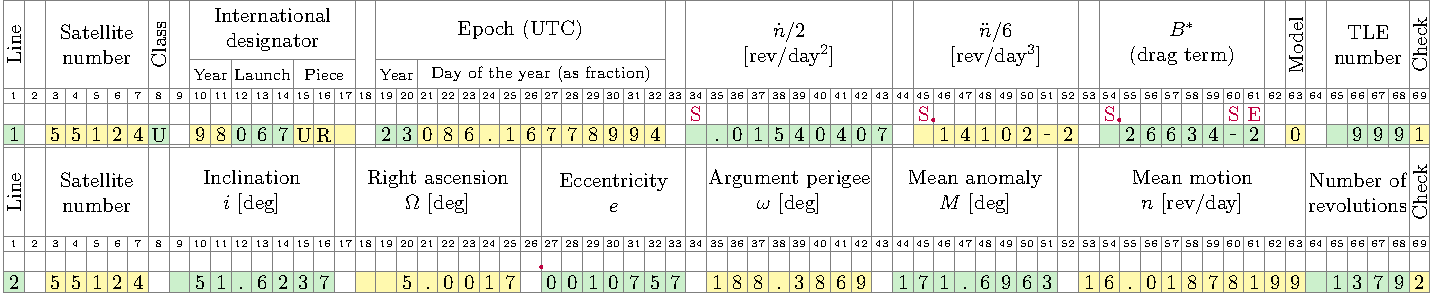
\includegraphics[width=\textwidth]{Images/TLE.pdf}
  \end{minipage}
  \caption{TLE data set from the NUTSAT satellite. The white (empty) cells designate space characters and the green and yellow ones are used to distinguish consecutive data blocks. The cells labeled with \textit{S} or \textit{E} respresent cells reserved for the negative sign and the exponent of a number respectively, while the red dots denote that an implicit decimal point is assumed.}
  \label{tab:TLE}
\end{table}
Let's clarify the meaning of some of the data blocks. The satellite number is a unique identifier assigned by NORAD ( \emph{North American Aerospace Defense Command}) for each earth-orbiting artificial satellite \cite{celestrak}. The classification of the satellite (Class) is divided into three categories: unclassified (U), classified (C), and secret (S). The international designator is comprised of three parts: the launch year (Year), the launch number of the year (Launch) and the piece of the launch (Piece). In the epoch year (Epoch), the first two numbers indicate the last two digits of the year, and the day of the year is represented as a fraction starting from 1. The model category refers to the orbital model used to generate the data, as specified in \cite{celestrak,wiki:spg}. The element set number (TLE number) is incremented by one when a new TLE (Two-Line Element) is generated for this satellite. On the second line, the number of revolutions indicates the number of times the satellite has orbited the Earth since its launch. Finally, the checksum (modulo 10) is used to verify the integrity of the data\footnote{Taking into account that the negative sign is counted as 1, and all the other cells without a number as 0.}.

\subsubsection{Position and velocity in terms of the TLEs' orbital elements}
We are now interested in proceed the other way around, that is, given the orbital elements or more precisely the TLE data, we want to compute the position and velocity of the satellite. In order to do that, we need to introduce the basis $(\vf{P}, \vf{Q}, \vf{W})$ linked to the orbit.
\begin{definition}[Perifocal coordinate system]\label{def:perifocal_coordinate_system}
  Consider the orbit of a satellite. We define its associated \emph{perifocal coordinate system} $(\vf{P},\vf{Q},\vf{W})$ as follows. The center is on the Earth's center of mass. The unit vectors $\vf{P}$ and $\vf{Q}$ lie on the orbital plane and are such that $\vf{P}$ points towards the periapsis, that is $\vf{P}:=\vf{B}/B$. The unit vector $\vf{W}$ is defined as $\vf{W}:=\vf{h}/h$, that is perpendicular to the orbital plane, and $\vf{Q}:=\vf{W}\times\vf{P}$.
\end{definition}
Recall that in \cref{sec:kepler_equation} we have seen that the position of the satellite in the perifocal frame is given by:
\begin{equation}
  \vf{r}_\mathrm{Peri} = a(\cos E-e)\vf{P} + a\sqrt{1-e^2}\sin E\vf{Q}
\end{equation}
Differentiating yields:
\begin{equation}
  \dot{\vf{r}}_\mathrm{Peri} = - a (\sin E)\dot{E}\vf{P}+a\sqrt{1-e^2}(\cos E)\dot{E}\vf{Q}
\end{equation}
where $\dot{E}=\frac{n}{1-e\cos E}$ is given by \cref{eq:kepler_equation_differential}. These two quantities depend on the two unknown variables $a$ and $E$, because $n$ and $e$ are given in the TLE data set. The semi-major axis can be easily obtained from $n$ due to the Kepler's third law (\cref{prop:kepler_third_law}). For the eccentric anomaly, we need to solve the Kepler equation:
\begin{equation}
  E-e\sin E = M
\end{equation}
\begin{lemma}
  Let $e\in[0,1)$, $M\in\RR$ and $\bar{M}=M\mod{2\pi}$ be such that $\bar{M}\in[0,2\pi)$. Then, the function
  \begin{equation}
    f(E) = E-e\sin E - M
  \end{equation}
  has a unique solution in the interval $[M, M+e]$ if $\bar{M}\in[0,\pi)$ and in the interval $[M-e, M]$ if $\bar{M}\in[\pi,2\pi)$.
\end{lemma}
\begin{proof}
  We first prove the uniqueness. Clearly $f\in\mathcal{C}^1(\RR)$ and $f'(E)=1-e\cos E> 0$ for all $E\in[0,2\pi)$ because $e<1$. Thus, $f$ is strictly increasing and so it has at most one zero. Now, if $0\leq \bar{M}< \pi$, then:
  \begin{equation}
    f(M)=-e\sin M\leq 0\qquad\text{ and }\qquad f(M+e)=e(1-\sin (M+e))\geq 0
  \end{equation}
  So by Bolzano's theorem, $f$ has a solution in $[M,M+e]$. If $\pi\leq \bar{M}< 2\pi$, then:
  \begin{equation}
    f(M)=-e\sin M\geq 0\qquad\text{ and }\qquad f(M-e)=-e(1+\sin (M-e))\leq 0
  \end{equation}
  So again by Bolzano's theorem, $f$ has a solution in $[M-e,M]$.
\end{proof}
We will use the Newton's method to find the zero of this non-linear equation. For small eccentricities $e$, the natural choice for the initial guess is $E_0=M$. For large eccentricities ($e>0.8$) the initial guess $E_0=\pi$ should be used in order to avoid convergency problems \cite{montenbruck}. Alternatively, we can do one or two steps of the bisection method to get a better initial guess, and then apply the Newton's method. Once obtained $E$, the position and velocity of the satellite in the J2000 frame are given by:
\begin{equation}
  \vf{r}_\mathrm{ECI} = \vf{T}\vf{r}_\mathrm{Peri} \qquad \dot{\vf{r}}_\mathrm{ECI} = \vf{T}\dot{\vf{r}}_\mathrm{Peri}
\end{equation}
where $\vf{T}$ is the rotation matrix that transform one frame to another and is given by (look at \cref{fig:orbital_elements}):
\begin{equation}
  \vf{T}=\vf{R}_z(-\Omega)\vf{R}_x(-i)\vf{R}_z(-\omega)
\end{equation}
\end{document}